\documentclass[a4paper]{article}

%====================== PACKAGES ======================

\usepackage[english]{babel}
\usepackage[utf8x]{inputenc}
%pour gérer les positionnement d'images
\usepackage{float}
\usepackage{amsmath}
\usepackage{graphicx}
\usepackage[colorinlistoftodos]{todonotes}
\usepackage{url}
%pour les informations sur un document compilé en PDF et les liens externes / internes
\usepackage{hyperref}
%pour la mise en page des tableaux
\usepackage{array}
\usepackage{tabularx}
%pour utiliser \floatbarrier
%\usepackage{placeins}
%\usepackage{floatrow}
%espacement entre les lignes
\usepackage{setspace}
%modifier la mise en page de l'abstract
\usepackage{abstract}
%police et mise en page (marges) du document
\usepackage[T1]{fontenc}
\usepackage[top=2cm, bottom=2cm, left=2cm, right=2cm]{geometry}
%Pour les galerie d'images
\usepackage{subfig}
%\usepackage{minted}
%\usepackage{subfigure}
%\usepackage{amsfonts}
\usepackage{enumitem}
\usepackage{amssymb}
\usepackage{pifont}
\usepackage{titlesec}
\usepackage{pdfpages}

\usepackage{indentfirst}


%====================== INFORMATION ET REGLES ======================

%rajouter les numérotation pour les \paragraphe et \subparagraphe
\setcounter{secnumdepth}{4}
\setcounter{tocdepth}{4}

\hypersetup{							% Information sur le document
pdfauthor = {Premier Auteur,
			},			% Auteurs
pdftitle = {Nom du Projet -
			Sujet du Projet},			% Titre du document
pdfsubject = {Mémoire de Projet},		% Sujet
pdfkeywords = {Tag1, Tag2, Tag3, ...},	% Mots-clefs
pdfstartview={FitH}}					% ajuste la page à la largueur de l'écran
%pdfcreator = {MikTeX},% Logiciel qui a crée le document
%pdfproducer = {}} % Société avec produit le logiciel

%======================== DEBUT DU DOCUMENT ========================

\begin{document}

%régler l'espacement entre les lignes
\newcommand{\HRule}{\rule{\linewidth}{0.5mm}}

%page de garde
\begin{titlepage}
\begin{center}

% Upper part of the page. The '~' is needed because only works if a paragraph has started.
%\includegraphics[width=0.7\textwidth]{figures/logo.jpg}~\\[1cm]



\textsc{\Large }\\[0.5cm]

% Title
\HRule \\[0.4cm]

{\huge \bfseries Rapport TP \\[0.4cm]
TL Traitement Du Signal \\[0.4cm] }

\HRule \\[4cm]

\begin{minipage}{0.7\textwidth}
  \begin{center} % Center the content within the minipage
    \LARGE
    \emph{Réalisé par:}\\
    Nabil \textsc{ABDELOUAHED}\\
    Yann \textsc{MARTIN}\\
  \end{center}
\end{minipage}
\begin{minipage}{0.4\textwidth}
  \begin{flushright} \large
    % Your content on the right if needed
  \end{flushright}
\end{minipage}
\vfill



% Bottom of the page
{\large \today}

\end{center}
\end{titlepage}

%page blanche
\newpage

\thispagestyle{empty}
\tableofcontents
\thispagestyle{empty}
\setcounter{page}{0}
%ne pas numéroter le sommaire



%espacement entre les lignes d'un tableau
\renewcommand{\arraystretch}{1.5}

%====================== INCLUSION DES PARTIES ======================

~

\newpage
\addcontentsline{toc}{section}{General Introduction}
\begin{center}
    {\huge \textbf{General Introduction}}\\
\end{center}

\vspace{1cm} 

In today’s digital landscape, the growth of small and medium-sized businesses,
particularly in the food and pastry industry, increasingly depends on their ability to establish
a strong online presence. Customers now expect the convenience of browsing products,
placing orders, and making secure payments online. Traditional pastry shops face the
challenge of adapting to this digital shift while preserving their artisanal identity and ensuring
a smooth user experience.\\

The Milanda Sweets pastry shop web application was conceived to address these
needs by providing a comprehensive eCommerce platform tailored for a traditional Tunisian
pastry shop. The platform aims to bridge the gap between the charm of artisanal sweets and
the efficiency of modern online shopping. By integrating intuitive browsing, real-time
updates, and secure transactions, the project empowers both the business and its customers
with a seamless digital experience.\\

The Milanda Sweets platform comprises two main components: a back-end system
responsible for managing products, users, orders, and analytics, and a front-end interface
designed for user engagement, product discovery, and online purchasing. Together, these
components deliver a responsive and functional system that simplifies operations for
administrators while enhancing convenience for end users.\\

This project is structured into three main chapters:
\begin{itemize}[label=\ding{51}]
    \item The first chapter, “Analysis and Preliminary Study,” explores the online pastry
market, identifies the shop’s needs, and defines the project’s core objectives and
functional requirements.
    \item The second chapter, “Conceptual Study,” presents the platform’s architectural
and technical design, including system modeling, database schema, and user flow.
    \item The third chapter, “Implementation,” details the development process,
technologies used, and the practical features that bring the platform to life—from
product management to real-time analytics and online payments.\\
\end{itemize} 

In conclusion, the Milanda Sweets pastry shop web application seeks to modernize the
customer experience and optimize business operations through a tailored digital solution. By
embracing web technologies, this platform enhances accessibility, increases efficiency, and
supports the long-term growth of a traditional pastry business in the digital era.


\newpage
\thispagestyle{empty} % This removes the page number
\vspace*{\fill}
\begin{center}
    {\Huge \textbf{Chapter 1:}}\\[0.8cm]
    {\Huge \textbf{Analysis and Preliminary Study}}
\end{center}
\vspace*{\fill}


\chapter{Analysis and Preliminary Study}
\addcontentsline{toc}{section}{Introduction}
{\Large \textbf{Introduction:}}\\

This introductory chapter aims to place the Milanda Sweets project within its general framework.\\

We will begin by presenting the project’s scope and the strategic importance it holds for both the business and its users. This will be followed by an overview of the existing situation and challenges facing traditional pastry businesses in the digital age. Then, we will conduct a detailed analysis of the functional and non-functional requirements, leading to a clear understanding of the project specifications. Finally, we will outline the methodology adopted to successfully execute the project.

\section{Project Overview:}

This work is part of the end-of-year project for the Software Engineering degree at
EPI Digital School for the academic year 2024/2025. It involves the independent research,
design, and development of a full-stack eCommerce web application tailored for a artisanal
pastry shop named Milanda Sweets.\\

The objective of the project is to support local businesses by providing a digital
platform that enhances their visibility, simplifies customer engagement, and streamlines
operations such as product management, order tracking, and secure payments. This solution
contributes not only to the modernization of small enterprises but also to meeting the
evolving expectations of today’s consumers who increasingly prefer online interactions.
The project aligns with the broader educational goals of applying theoretical knowledge to
real-world scenarios, using modern development tools and best practices in software
engineering.

\section{Study of Existing Solutions:}

To ensure the quality and uniqueness of Imagify, a study of existing solutions in the
field of text-to-image generation was conducted. This section explores prominent solutions,
highlighting their advantages and limitations.

\subsection{Pâtisserie Mme Masmoudi:}

Masmoudi is the hallmark of fine gastronomy and the embodiment of a passed-down
heritage. A fine pastry shop founded in 1972 in Sfax [1].

\begin{figure}[!h]
\begin{center}
\includegraphics[width=15cm]{images/Pâtisserie Mme Masmoudi.png}
\end{center}
\caption{Pâtisserie Mme Masmoudi}
\end{figure}

\newpage
\subsection{Gourmandise:}

Gourmandise Tunisian Pastry, the shop was founded in 1976. It specializes in Tunisian, Western, and Eastern cakes and savory pastries [2].

\begin{figure}[!h]
\begin{center}

\includegraphics[width=15cm]{images/Gourmandise.png}
\end{center}
\caption{Gourmandise}
\end{figure}

\subsection{Pâtisserie Mme Rekik:}

At the Maison, Mrs. REKIK is a quality label rooted in tradition, which she strives to perpetuate with an appropriate dose of modernity [3].

\begin{figure}[!h]
\begin{center}
\includegraphics[width=15cm]{images/Pâtisserie Mme Rekik.png}
\end{center}
\caption{Pâtisserie Mme Rekik}
\end{figure}

\newpage
\section{Critique of Existing Solutions:}

Despite these pastry shops being well-regarded for their traditional Tunisian pastries, their websites face several challenges in terms of customer experience:\\


\textbf{Pâtisserie Mme Masmoudi:}\\

\begin{itemize}[label=\textbullet]
    \item The website lacks a user-friendly interface, which can make navigation cumbersome for customers seeking specific products quickly. This can lead to frustration and a longer browsing experience.
    \item No integration with social media platforms, reducing the potential for engaging with customers through promotions or direct interaction.\\
\end{itemize}

\textbf{Gourmandise:}\\

\begin{itemize}[label=\textbullet]
    \item The platform is heavily reliant on bulk production methods, which does not align with the handcrafted nature of Patisserie Artisanal Tunisienne.
    \item Customization in product presentation and limited direct customer interaction reduce the ability to highlight the authenticity and craftsmanship behind each pastry.\\
\end{itemize}

\textbf{Pâtisserie Mme Rekik:}\\

\begin{itemize}[label=\textbullet]
    \item Navigation on the site is not as intuitive as it could be. Categories for different types of pastries are not clearly defined, making it harder for users to find specific products or explore the full range of offerings.
    \item There’s no e-commerce functionality, meaning customers cannot place online orders or arrange for delivery, limiting convenience for those who want to shop from home.
\end{itemize}

\section{Our solution:}

Based on an in-depth analysis of existing platforms and the specific functional needs identified for our project, we propose the development of a comprehensive digital solution: a mobile and web application dedicated to showcasing and facilitating access to Tunisian artisanal pastries.\\

Our goal is not only to simplify the process of ordering pastries but also to deliver a personalized and memorable experience for every user. Through a user-friendly interface, tailored recommendations, and modern features, we aim to turn every interaction into a delightful moment.\\

The application is divided into two core spaces:\\

\begin{itemize}[label=\textbullet]
    \item \textbf{Admin Dashboard:} A powerful back-office panel to manage products, orders, users, and performance analytics.
    \item \textbf{Customer Space:} A welcoming environment for exploring pastries, placing orders, and receiving personalized recommendations.
\end{itemize}


\section{Requirements Analysis:}

A software requirements analysis is a detailed description of the system to be developed, including its functional and non-functional requirements. This analysis serves as the foundation for agreements between stakeholders regarding the expected functionality and operation of the software.

\subsection{Actors Identification:}

For Milanda Sweets eCommerce platform, the following actors are identified:\\

\textbf{Visitor:}  is someone who visits the website without logging in. They can browse the products, learn about the pastries offered, and view general information about the store.\\

\textbf{Customer:}  is a registered user who can make purchases, track orders, and receive notifications about new products and promotions.\\                      

\textbf{Admin:}  is responsible for managing the website content, overseeing customer interactions, and ensuring that the eCommerce platform runs smoothly.\\

\subsection{Functional Requirements:}

Below are the functional requirements for each of the identified actors in the system:\\

\textbf{Visitor:}\\

\begin{itemize}[label=\textbullet]
    \item Access general information about the store.
    \item Register or log in to become a customer.\\
\end{itemize}
        
\textbf{Customer:}\\

\begin{itemize}[label=\textbullet]
    \item Browse pastries based on categories or preferences.
    \item Add products to the cart and proceed to checkout.
    \item Place orders and make payments through the website.
    \item Manage their account.
    \item Receive order confirmations and shipping updates.
    \item Add products to the wish-list.\\
\end{itemize}

\newpage
\textbf{Admin:}\\

\begin{itemize}[label=\textbullet]
    \item Manage products.
    \item Manage orders.
    \item Manage customer’s requests.
    \item Manage content.
\end{itemize}

\subsection{Non Functional Requirements:}

Non-functional requirements define system attributes that ensure overall system quality. The Pâtisserie Artisanal Tunisienne eCommerce platform must adhere to the following:\\

\textbf{Performance:}\\

\begin{itemize}[label=\textbullet]
    \item The system should be responsive and handle concurrent users efficiently, especially during peak times.
    \item The website should load in 2-3 seconds for an optimal user experience.\\
\end{itemize}
        
\textbf{Reliability:}\\

\begin{itemize}[label=\textbullet]
    \item The system must have high availability with minimal downtime, ensuring continuous service.
    \item Regular updates should occur without disrupting user experience.\\
\end{itemize}

\textbf{Usability:}\\

\begin{itemize}[label=\textbullet]
    \item The platform should be intuitive with easy navigation, simple product search, and a smooth checkout process.
    \item The admin panel should be easy to use for managing products, orders, and customer data.\\
\end{itemize}

\textbf{Data Integrity:}\\

\begin{itemize}[label=\textbullet]
    \item The system must maintain accurate and consistent product, order, and customer data, with regular backups and transactional databases to ensure data protection.
\end{itemize}

\section{Working Methodology:}

In the context of our project, we adopted the Iterative-Incremental methodology,
guided by Agile principles, following the definition of our objectives. Unlike rigid models
such as the V-Model or Waterfall, the iterative approach allowed us to develop the
application in functional segments, test frequently, and adapt to evolving requirements
throughout the project lifecycle. The methodology operates across two interrelated phases: Planning and Design, and
Development and Testing.\\

\textbf{Planning and Design Phase:}\\

This phase focuses on understanding the client’s needs, analyzing the market and
competitors, defining the core features, and designing the system architecture and database schema.
Wireframes, UI mockups, and data models were created to guide the implementation process
and reduce ambiguity.\\

\textbf{Development and Testing Phase:}\\

This phase follows an incremental delivery strategy, where the system was developed
in small functional units (product catalog, cart system, checkout, admin dashboard, etc.).
Each unit underwent implementation, testing, and review.
Throughout this process, feedback loops were integrated to ensure continuous improvement
and refinement of features.
Testing (manual and functional) was carried out regularly to maintain software reliability and
quality.

\begin{figure}[!h]
\begin{center}
\includegraphics[width=15cm]{images/Iterative-Incremental process.png}
\end{center}
\caption{Iterative-Incremental Process}
\end{figure}


\section{Planning:}

This project spanned a period of 70 days (4 months + 10 days), from January 1st, 2025, to May 5th, 2025. To move from conceptualization to implementation, it was essential to establish clear objectives within a defined timeline. To manage the complexity of the project over time, each stage was outlined in a detailed calendar format, allowing us to track progress and evaluate if we were on schedule or experiencing delays.\\

For effective project management, we employed a Gantt chart to visualize and plan the different stages of the project, which included research, design, development, and report writing. The planning process was structured as follows:\\

\textbf{Research Phase:}\\

The initial phase involved conducting thorough research to understand the needs of the pastry business, industry trends, and best practices in eCommerce. This phase laid the foundation for informed decision-making throughout the project.\\

\textbf{Analysis and Requirement Specification:}\\

In this phase, we focused on gathering and analyzing the project’s functional and non-functional requirements. This included understanding the specific needs of the Milanda Sweets business, defining user roles, and setting clear objectives for the platform (e.g., product catalog, payment integration, admin panel, etc.).\\

\textbf{Design Phase:}\\

Once the requirements were defined, we moved on to the design phase, where we created detailed use case diagrams, class diagrams, and UI/UX wireframes. This phase was crucial for visualizing the platform’s structure and ensuring that the design met the functional goals of the project.\\

\textbf{Development Phase:}\\

In the development phase, we focused on learning the necessary technologies (MERN stack) and began coding the application. This phase involved developing both the frontend (React.js, Tailwind CSS) and the backend (Node.js, Express, MongoDB), integrating key features such as product listing, shopping cart, user authentication, and payment gateways.\\

\textbf{Report Writing:}\\

Throughout the development process, the project report was continuously updated to document the progress, challenges, and milestones. The final phase involved compiling these insights into a comprehensive report, which was finalized at the conclusion of the project.\\

\begin{figure}[!h]
\begin{center}
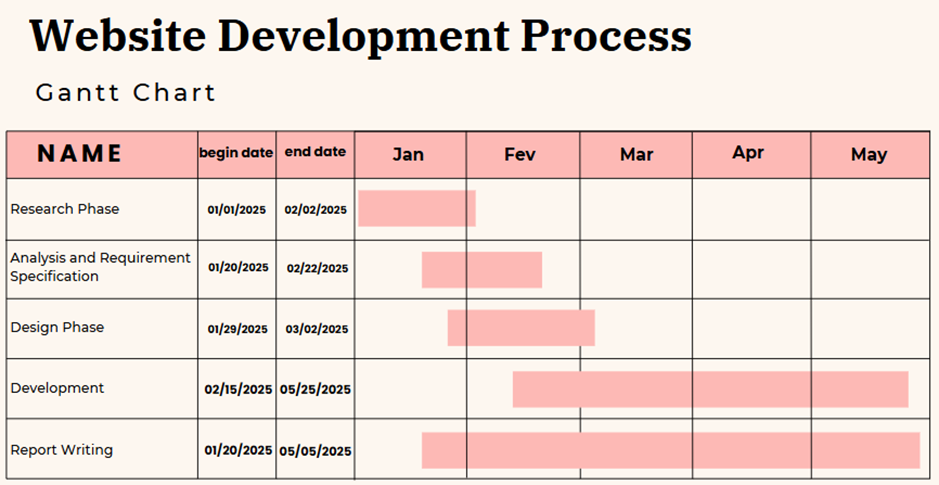
\includegraphics[width=15cm]{images/Gantt diagram.png}
\end{center}
\caption{Gantt diagram}
\end{figure}


\addcontentsline{toc}{section}{Conclusion}
{\Large \textbf{Conclusion:}}\\

In this chapter we analyzed the existing landscape by exploring similar pastry shop and eCommerce solutions already available in the market , we also identified the main actors involved in the system, detailed both functional and non-functional requirements which allowed us to identify gaps and propose our own tailored solution for Milanda Sweets .Moreover we defined the methodology adopted for our project and outlined a structured planning approach to guide the project from research through to development and reporting.
The next chapter will focus on the conceptual design of our proposed solution, including system architecture and detailed modeling.

\newpage
\thispagestyle{empty}
\vspace*{\fill}
\begin{center}
    {\Huge \textbf{Chapter 2:}}\\[0.8cm]
    {\Huge \textbf{Conceptual Study}}
\end{center}
\vspace*{\fill}


\chapter{Conceptual Study}

\addcontentsline{toc}{section}{Introduction}
{\Large \textbf{Introduction:}}\\

This chapter focuses on the design phase of our application, which forms the essential groundwork for the development process. Here, we present the design approach adopted and introduce a series of diagrams that illustrate the structural and behavioral aspects of the system. This comprehensive design ensures that the final implementation remains aligned with the project’s objectives.

\section{Design Methodology:}

For the design of our system, we adopted UML (Unified Modeling Language) a widely used object-oriented modeling standard. UML allows for the visualization of software architecture using a variety of diagram types, making it easier to specify the system’s structure, behavior, and interactions.\\

By translating complex technical specifications into intuitive diagrams, UML plays a crucial role in enhancing clarity and communication among stakeholders. It serves as a visual language that reduces the need for lengthy textual descriptions and makes the system design more accessible and maintainable.

\section{Use Case Diagrams:}

Use case diagrams provide a high-level overview of the system by illustrating how different users (actors) interact with the application's functionalities (use cases). These diagrams help to define the system's scope and identify the core interactions between users and the system.

\subsection{Global Use Case Diagram:}

The following diagram presents a global view of the main use cases within our application. It captures the primary actors such as administrators, customers and highlights their respective interactions with the system. This global perspective offers a clear understanding of the application's functional boundaries and user engagement.\\

\newpage
\begin{figure}[!h]
\begin{center}
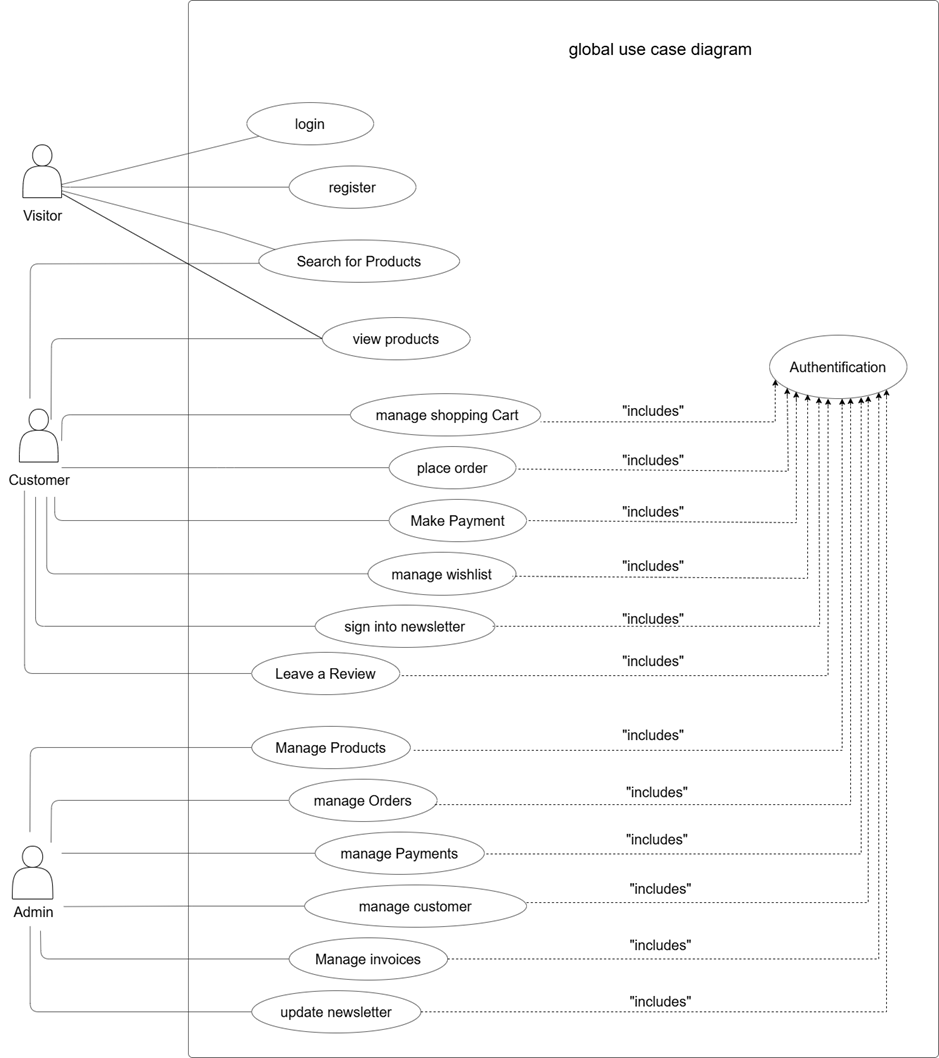
\includegraphics{images/Global Use Case Diagram.png}
\end{center}
\caption{Global Use Case Diagram}
\end{figure}


\subsection{Refined Use Case Diagrams:}

\underline{\textbf{Place Order Use Case Diagram:}}\\

In the following use case diagram, we detail the process that takes place in order for  the customer to place the order.\\

\newpage
\begin{figure}[!h]
\begin{center}
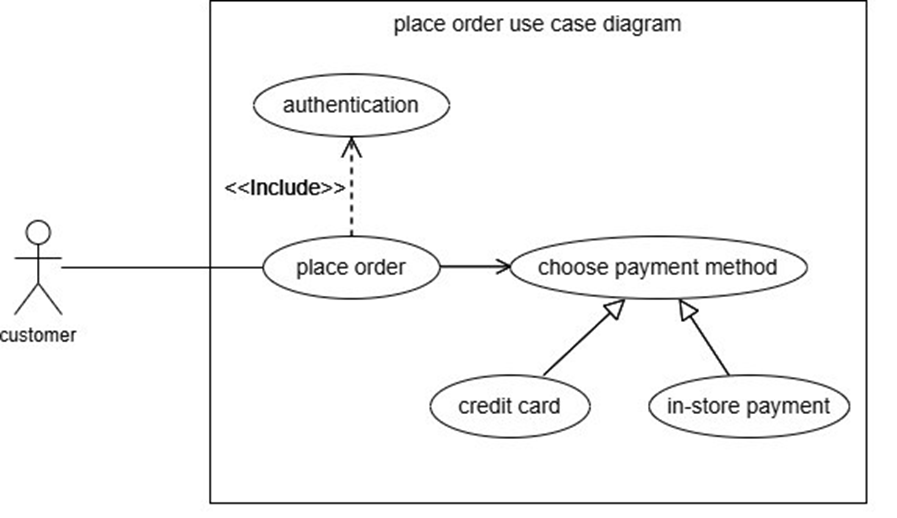
\includegraphics[width=13cm]{images/Place Order Use Case Diagram}
\end{center}
\caption{Place Order Use Case Diagram}
\end{figure}

\underline{\textbf{Product Management Use Case Diagram:}}\\

In this use case diagram we could see the various possible actions of the ”admin Product Managment ” in order to manage products.\\

\begin{figure}[!h]
\begin{center}
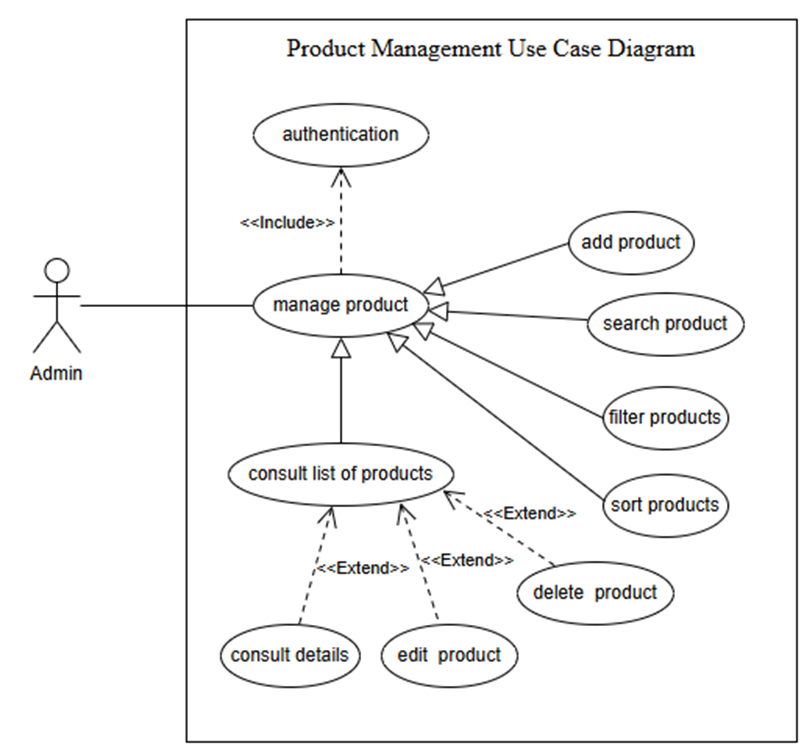
\includegraphics[width=13cm]{images/Product Management Use Case Diagram.png}
\end{center}
\caption{Product Management Use Case Diagram}
\end{figure}

After authentication, the user with the role of "Admin" can access the product management interface. From this interface, the admin can perform core operations such as adding a new product by providing its name, category, description, images, price, and stock details. The admin can also browse the existing product list, apply filters for easier navigation, and either update product information or remove a product entirely from the system. These actions ensure that the product catalog remains accurate, up to date, and reflective of the current inventory and offerings.\\

\underline{\textbf{Cart Management Use Case Diagram:}}\\

In the following use case diagram, we detail possible actions that could be done by the customer in order to manage the cart.\\

\begin{figure}[!h]
\begin{center}
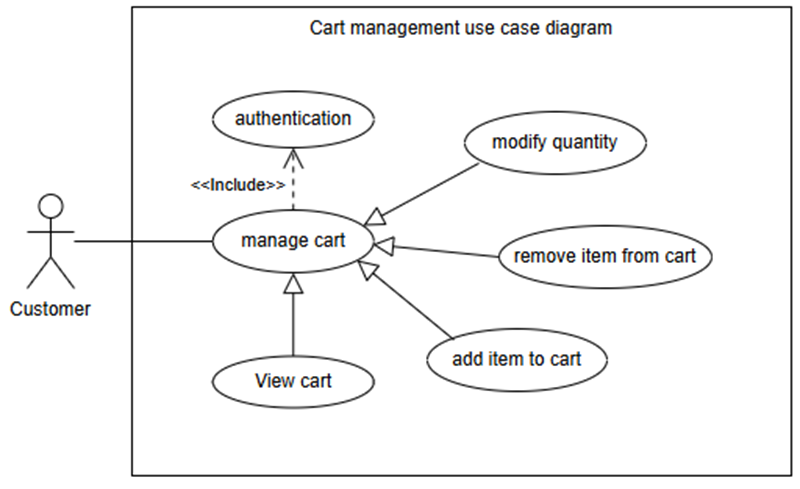
\includegraphics[width=14cm]{images/Cart Managment Use Case Diagram.png}
\end{center}
\caption{Cart Management Use Case Diagram}
\end{figure}

After authentication, the user with the role of "Customer" can manage the contents of their shopping cart through a dedicated interface. The user can add products to the cart from the product listing or detail pages, specifying the desired quantity. They can view a summary of all items in the cart, update quantities, or remove products entirely. The system automatically recalculates the total price after each change.This use case ensures a smooth and flexible shopping experience prior to placing an order.

\section{Classes Diagram:}

The class diagram illustrates the static structure of the Milanda Sweets system. It models the core entities (classes) within the application, detailing their attributes, methods, and the relationships that connect them. Each user is associated with a specific role defined by the role attribute in the User class, which may be a “Customer” or “Admin” .These roles determine access rights and functionalities across the platform, such as placing orders, managing products, or overseeing system users.\\

The figure below represents the class diagram of our application.\\

\begin{figure}[!h]
\begin{center}
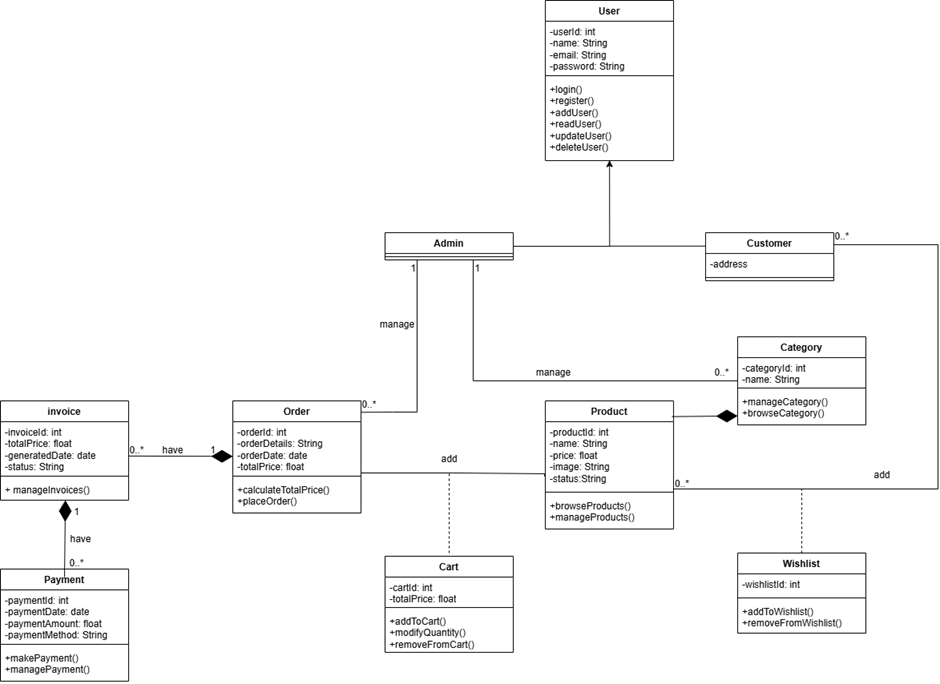
\includegraphics{images/Global Class Diagram.png}
\end{center}
\caption{Global Class Diagram }
\end{figure}

\newpage
\section{Sequence Diagram:}

A sequence diagram illustrates the interactions between objects in a system, presented in the order they occur. It showcases how objects work together and the sequence of their actions.

\subsection{"Login" Sequence Diagram:}

To log in, the user provides a username and password. The front-end validates the input format and length before sending a POST request to the /Login endpoint. The server uses Mongoose to check if the user exists. If not, it responds with a 401 Unauthorized status. If the user is found, the server verifies the password using bcrypt. On success, it generates a session or token and sends it back with user details. The client stores the authentication data and redirects the user to the home page, completing the login process.

\newpage
\begin{figure}[!h]
\begin{center}
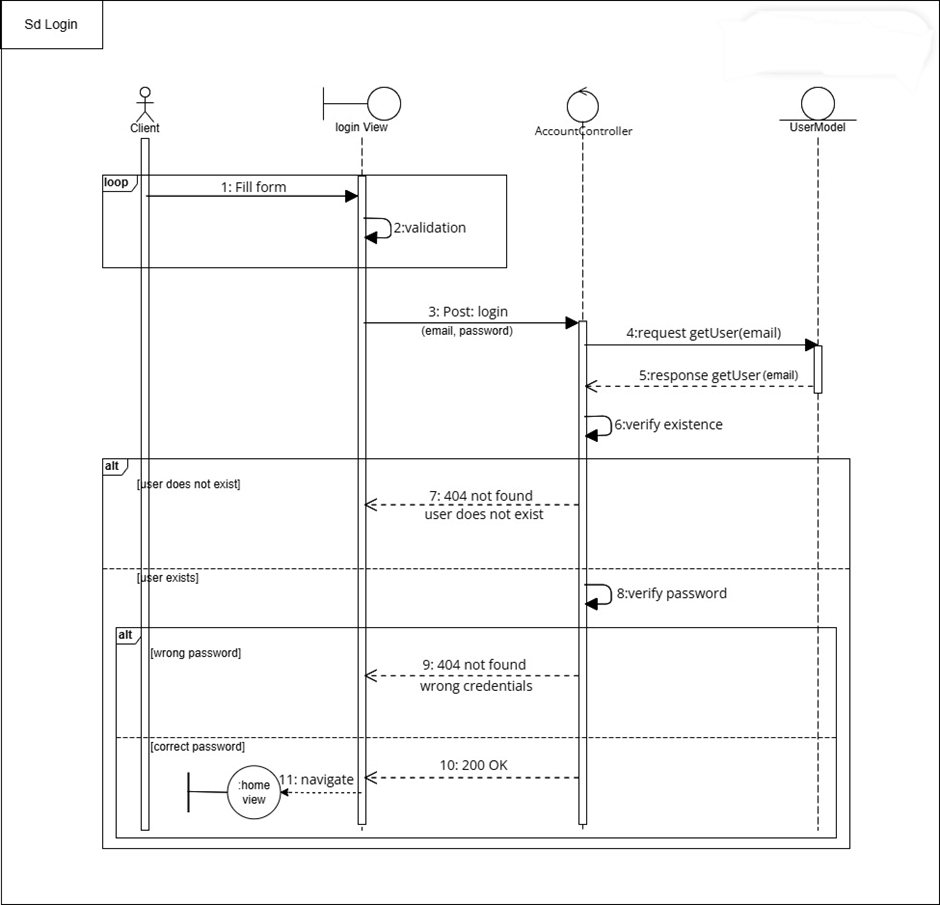
\includegraphics{images/Login Sequence Diagram.png}
\end{center}
\caption{Login Sequence Diagram}
\end{figure}

\subsection{"Placing order" Sequence Diagram:} 

To place an order, the user must be logged in. From the front end, the customer selects products and adds them to the cart. Once ready, the user initiates checkout, prompting the interface to collect delivery and payment details. These details are sent via a POST request to the /orders endpoint. The server verifies product availability using Mongoose queries and confirms stock levels. If all items are available, the system processes the payment using a secure payment gateway. Upon successful payment, the backend creates an order document in the database, assigns it to the user, and clears the cart. The client receives an order confirmation response and redirects the user to an order success page, completing the transaction flow.

\newpage
\begin{figure}[!h]
\begin{center}
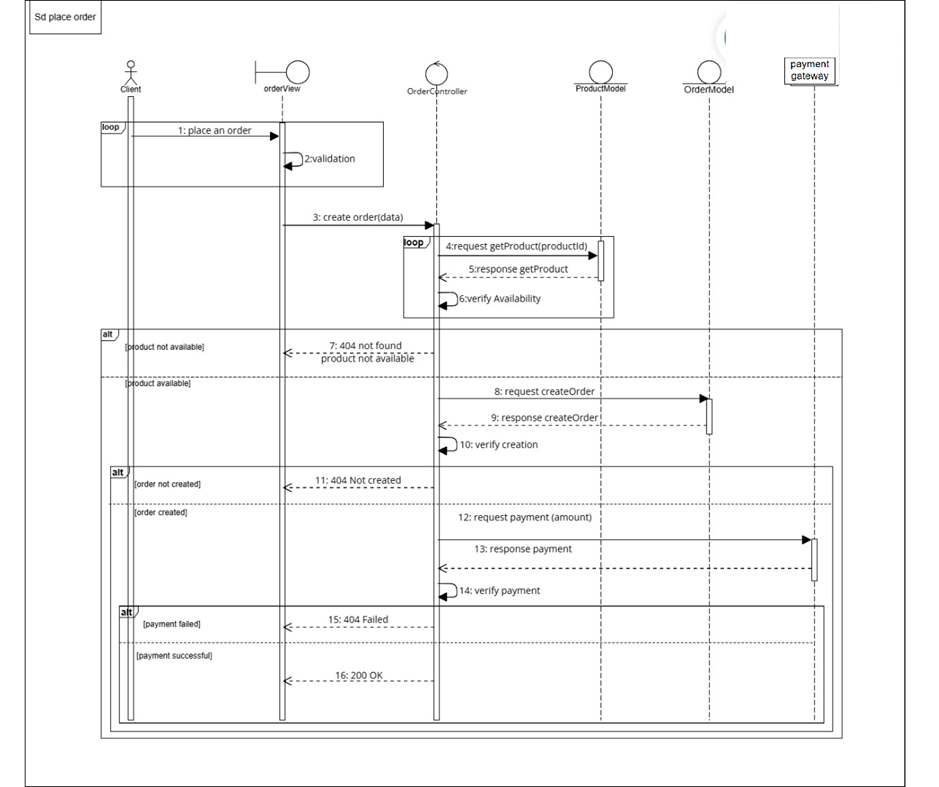
\includegraphics{images/Placing Order Sequence Diagram.png}
\end{center}
\caption{Placing Order Sequence Diagram}
\end{figure}

\addcontentsline{toc}{section}{Conclusion}
{\Large \textbf{Conclusion:}}\\

In this chapter, we focused on the essential phase of system design for our eCommerce platform, Milanda Sweets. We began by adopting the UML methodology to guide our design process. This included developing use case diagrams to represent the interactions between different actors such as customers, admins, and guests and the main functionalities of the system.\\

We then constructed a class diagram to define the structural blueprint of our application, highlighting the key classes involved, such as products, users, orders, and their relationships. Lastly, we created sequence diagrams to visualize the step-by-step flow of interactions between the system’s components during key operations like order placement and user authentication.
With the system’s behavior, structure, and dynamic interactions clearly defined, we are now ready to proceed to the implementation phase, which will be covered in the next chapter.

\newpage
\thispagestyle{empty}
\vspace*{\fill}
\begin{center}
    {\Huge \textbf{Chapter 3:}}\\[0.8cm]
    {\Huge \textbf{Implementation}}
\end{center}
\vspace*{\fill}


\chapter{Implementation}

\addcontentsline{toc}{section}{Introduction}
{\Large \textbf{Introduction:}}\\

In this final chapter, we concentrate on the implementation phase, the concluding step in software development. This stage involves coding the application. We begin by outlining the global architecture and selecting the appropriate technologies, concluding with an overview of our solution presented through screenshots.\\

\section{System Architecture:}

Before we get into the chosen technologies, it is beneficial to take a look at the architecture that composes our system.

\subsection{N-tier architecture:}

N-tier architecture, also known as multi-layer architecture, is a client-server model that divides system responsibilities across separate layers. Typically, it includes three primary tiers: presentation, business logic, and data.\\

This clear separation of concerns enhances scalability and simplifies software maintenance.

\begin{itemize}[label=\textbullet]
    \item \textbf{Presentation Tier:} The client-facing layer responsible for the user interface, allowing users to interact with the system.
    \item \textbf{Business Logic Tier:} The layer where the core system logic resides, acting as an intermediary between the user interface and the database.
    \item \textbf{Data Tier:} The backend layer that handles data storage and management, often using a database system.
\end{itemize}

The following is a diagram of the representation of the 3 tiers in our application:

\begin{figure}[!h]
\begin{center}
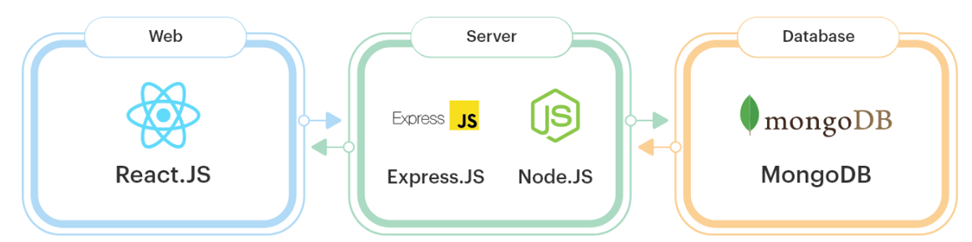
\includegraphics{images/Tier Architecture.png}
\end{center}
\caption{Tier Architecture}
\end{figure}

\subsection{MVC Pattern:}

The Model-View-Controller (MVC) pattern is a widely used software design pattern for building user interfaces. It separates concerns, dividing data presentation, user interaction, and system logic. MVC is popular in web development, with dedicated frameworks available for most programming languages. Here's a breakdown of its components:

\begin{itemize}[label=\textbullet]
    \item \textbf{Model:} Represents the application's data, often linked to database tables.
    \item \textbf{View:} The user interface, such as web pages in a web application.
    \item \textbf{Controller:} Manages system logic and facilitates communication between the Model and View.
\end{itemize}

\begin{figure}[!h]
\begin{center}
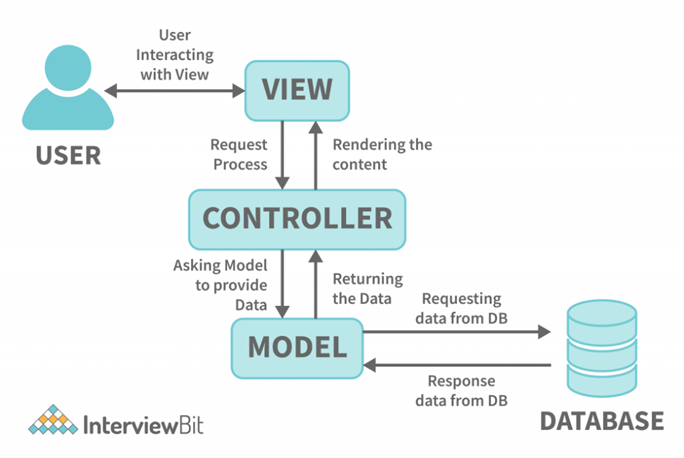
\includegraphics[width=12cm]{images/Interaction within MVC.png}
\end{center}
\caption{Interaction within MVC}
\end{figure}

\section{Framework:}

The selection of technologies is a critical step before starting application development. It is essential to thoroughly evaluate and compare various technologies to choose the most suitable ones that ensure optimal application performance.

\subsection{React.js:}

\begin{figure}[!h]
\begin{center}
\includegraphics[width=5cm]{images/Reactjs.png}
\end{center}
\caption{React.js}
\end{figure}

A JavaScript library for building user interfaces. React makes it painless to create interactive UIs. Design simple views for each state in your application, and React will efficiently update and render just the right components when your data changes [4].

\subsection{Express.js:}

\begin{figure}[!h]
\begin{center}

\includegraphics[width=6cm]{images/Expressjs.png}
\end{center}
\caption{Express.js}
\end{figure}

Express.js is a framework for building web applications based on Node.js. It is, in fact, the standard framework for server-side development in Node.js [5].

\subsection{Tailwind.css:}

\begin{figure}[!h]
\begin{center}

\includegraphics[width=6cm]{images/Tailwind.png}
\end{center}
\caption{Tailwind.css}
\end{figure}

Tailwind CSS is an open-source CSS framework. Unlike other CSS frameworks such as Bootstrap, its main feature is that it does not offer a predefined set of component classes. Instead, it provides low-level utility classes that can be combined to create custom designs directly in the HTML structure, offering greater flexibility and control over the styling [6].

\subsection{Mongoose:}

\begin{figure}[!h]
\begin{center}

\includegraphics[width=6cm]{images/Mongoose.png}
\end{center}
\caption{Mongoose}
\end{figure}

Mongoose is an object-oriented JavaScript library that creates a connection between MongoDB and the JavaScript runtime environment Node.js [7].

\section{Software Tools:}

\subsection{Node.js:}

\newpage
\begin{figure}[!h]
\begin{center}

\includegraphics[width=5cm]{images/Node.png}
\end{center}
\caption{Node.js}
\end{figure}

Node.js is a free, open-source, cross-platform JavaScript runtime environment that lets developers create servers, web apps, command line tools and scripts [8].

\subsection{GitHub:}

\begin{figure}[!h]
\begin{center}

\includegraphics[width=6cm]{images/github.png}
\end{center}
\caption{GitHub}
\end{figure}

GitHub, Inc. is a software development and services company in the United States. GitHub specifically develops the GitHub platform and the Electron framework [9].

\subsection{Postman:}

\begin{figure}[!h]
\begin{center}

\includegraphics[width=6cm]{images/Postman.png}
\end{center}
\caption{Postman}
\end{figure}

Postman is an application used to test APIs, created in 2012 by Abhinav Asthana, Ankit Sobti, and Abhijit Kane in Bangalore to address the issue of shareable API testing [10].

\subsection{Lucidchart:}

\begin{figure}[!h]
\begin{center}

\includegraphics[width=6cm]{images/Lucidchart.png}
\end{center}
\caption{Lucidchart}
\end{figure}

Lucidchart is an online collaboration platform, cloud-based, enabling the creation of diagrams, data visualization, and other conceptual schematics [11].

\subsection{Visual Studio Code:}

\begin{figure}[!h]
\begin{center}

\includegraphics[width=4cm]{images/vsc.png}
\end{center}
\caption{Visual Studio Code}
\end{figure}

Visual Studio Code is an extensible code editor developed by Microsoft for Windows, Linux, and macOS.\\

Its features include support for debugging, syntax highlighting, intelligent code completion (IntelliSense), snippets, code refactoring, and built-in Git. Users can customize the theme, keyboard shortcuts, preferences, and install extensions that add additional functionality [12].

\section{Database:}

\subsection{MongoDB:}

\begin{figure}[!h]
\begin{center}
\includegraphics[width=6cm]{images/mongodb.png}
\end{center}
\caption{MongoDB}
\end{figure}

MongoDB Atlas integrates operational and vector data in a single, unified platform. Use vector representations of your data to perform semantic search, build recommendation engines, design Q\&A systems, detect anomalies, or provide context for gen AI Apps [13].

\section{User Interfaces:}

In this section, we will showcase some key interfaces of our solution, highlighting the most important features of our work.

\subsection{Hompage:}

The homepage serves as the main entry point of our platform, offering users an overview of the available features and quick access to essential sections of the site, we will find some tranding product along side with the available categories. It also contains the services this pastry shop offers. It is publicly accessible, allowing visitors to explore the content without needing to log in.

\begin{figure}[!h]
\begin{center}

\includegraphics{images/Homepage.png}
\end{center}
\caption{Homepage}
\end{figure}

\newpage
\subsection{Registration:}

This figure shows the registration page of the application. New users can create an account by providing the required information, such as their name, email address, and password. Upon submission, the data is securely transmitted to the server, where the password is encrypted. Once registration is successful, the user can log in and access the platform with permissions based on their assigned role.

\begin{figure}[!h]
\begin{center}
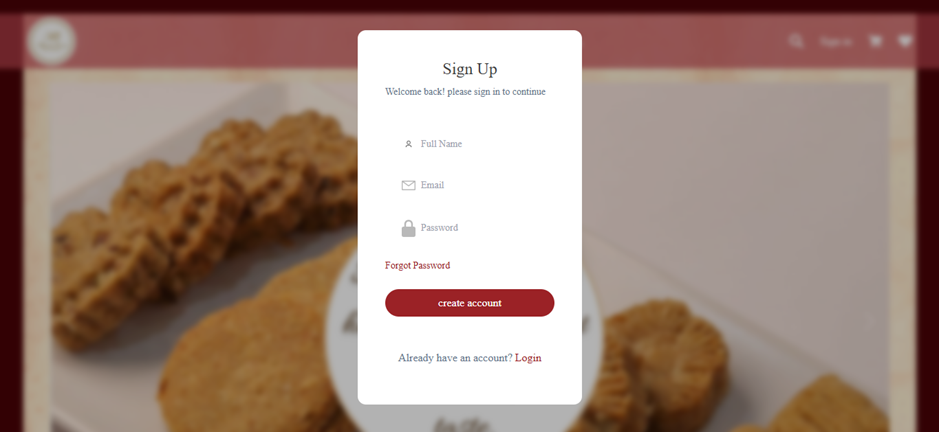
\includegraphics{images/Registration.png}
\end{center}
\caption{Registration}
\end{figure}

\subsection{Authentication:}

The figure below illustrates the application's login page. Each user can authenticate by entering their email address and password. These credentials are then sent to the server, where the password is encrypted for security purposes. Once the email and password are verified, the user is redirected to their account with access tailored to their specific role within the application.

\begin{figure}[!h]
\begin{center}
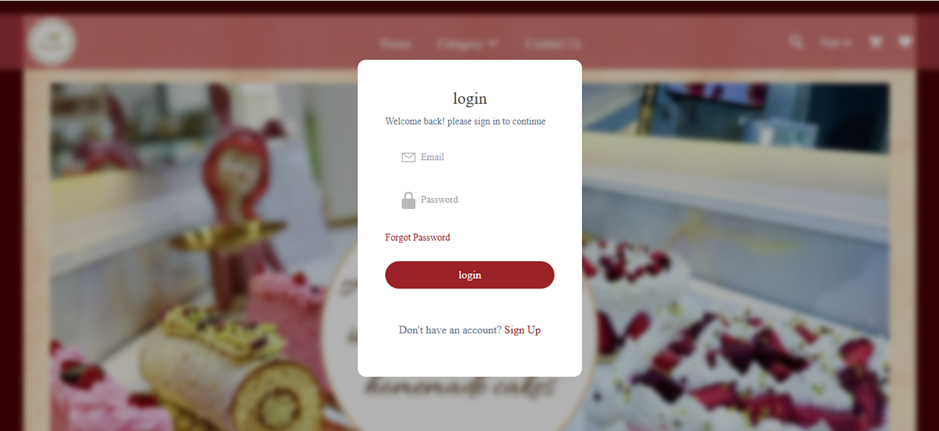
\includegraphics{images/Authentication.png}
\end{center}
\caption{Log in}
\end{figure}

\newpage
\subsection{Products page:}

This page presents users with a curated list of products grouped under a selected category,When a user selects a category from the menu, a request is sent to the server to retrieve all products belonging to that category. The server responds with the relevant data, which is then dynamically rendered as a grid of product cards displaying key details like the product name, image, and price. Users can further refine their browsing experience using built-in filtering and sorting options such as sorting by price or filtering by availability making it easier to discover products that match their preferences.

\begin{figure}[!h]
\begin{center}
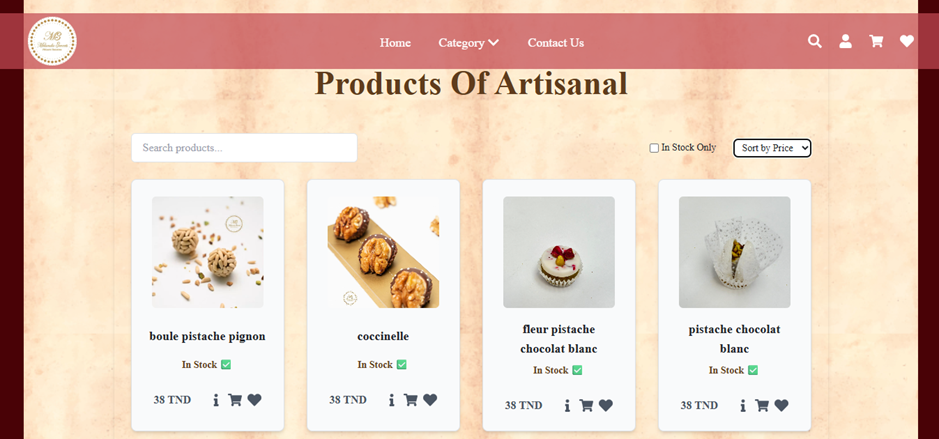
\includegraphics{images/products.png}
\end{center}
\caption{Products page}
\end{figure}

\subsection{Product details page:}

When a user clicks on the details button of a product a request is sent to the server to retrieve complete details of that item. The response includes elements like a rich description, list of ingredients, corresponding category, price, and current availability along side with an image. Users can review the pastry in detail and easily add it to their cart for purchase, making the browsing and ordering experience smooth and delightful.

\begin{figure}[!h]
\begin{center}

\includegraphics{images/product details.png}
\end{center}
\caption{Product details}
\end{figure}

\subsection{Shopping cart page:}

The shopping cart page allows users to review and manage their selected pastry items before placing an order. When a user adds a product to the cart it appears in a detailed list displaying the product name, selected quantity, individual price, and subtotal. Users can adjust quantities or remove items. The page also provides an automatically updated total price.This step ensures that customers can verify their selections and proceed confidently to finalize their order.

\begin{figure}[!h]
\begin{center}
\includegraphics{images/Shopping cart page.png}
\end{center}
\caption{Shopping cart page}
\end{figure}

\subsection{Wishlist page:}

The wishlist page lets users save their favorite pastries for future purchase. When a user adds a product to their wishlist, it’s stored for easy access later. Each item in the wishlist displays the product name, price, and an option to quickly add it to the cart. Users can remove items, view details, or check availability. This page offers a convenient way for customers to keep track of items they want to purchase, making it easier to return to their desired products whenever they're ready to place an order.

\begin{figure}[!h]
\begin{center}
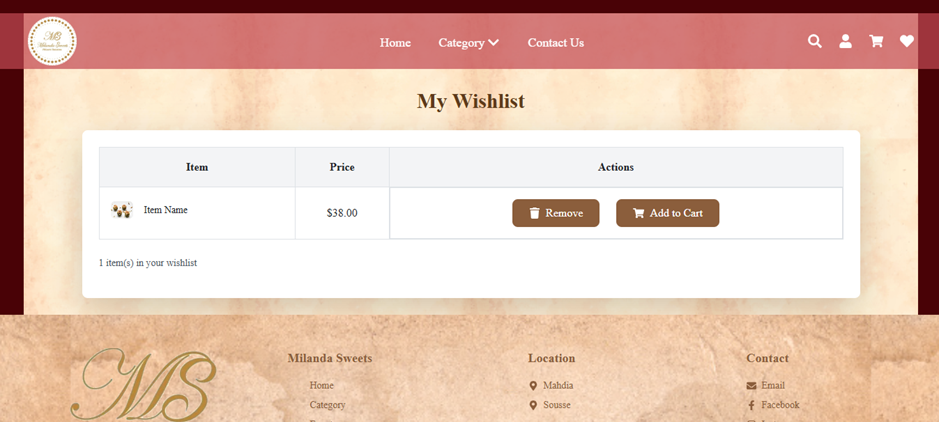
\includegraphics{images/Wishlist.png}
\end{center}
\caption{Wishlist}
\end{figure}

\subsection{Checkout Page:}

The checkout page guides users through the final steps of placing their order. It is divided into multiple components, each handling a specific part of the process. This structured flow ensures a smooth and secure checkout experience, allowing customers to confirm all necessary details before completing their pastry order.

\begin{figure}[!h]
\begin{center}
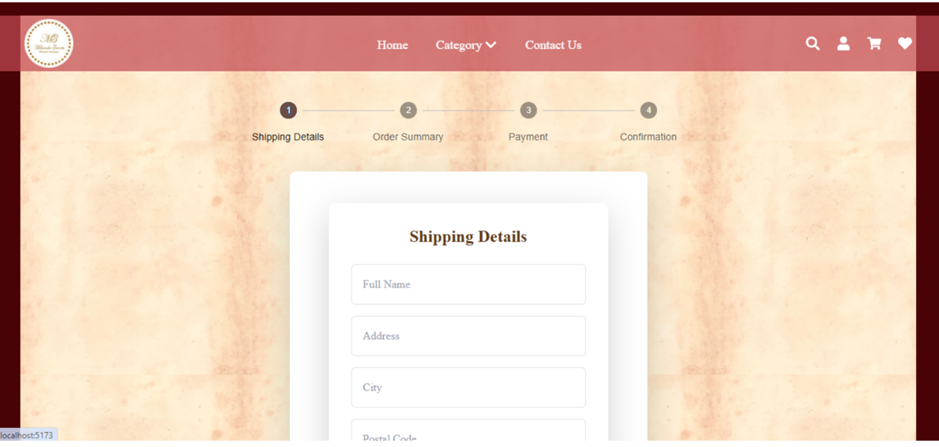
\includegraphics{images/checkout page.png}
\end{center}
\caption{Checkout page}
\end{figure}

\textbf{Shipping details:}\\

The Shipping Details section collects the delivery information needed to fulfill the customer’s order. Users are prompted to enter essential details such as their full name, phone number, address, city, and postal code. The form ensures that all required fields are validated
before proceeding, reducing the risk of delivery errors. This information is securely handled and used solely for the purpose of ensuring timely and accurate delivery of the selected pastries to the customer's specified location.

\begin{figure}[!h]
\begin{center}
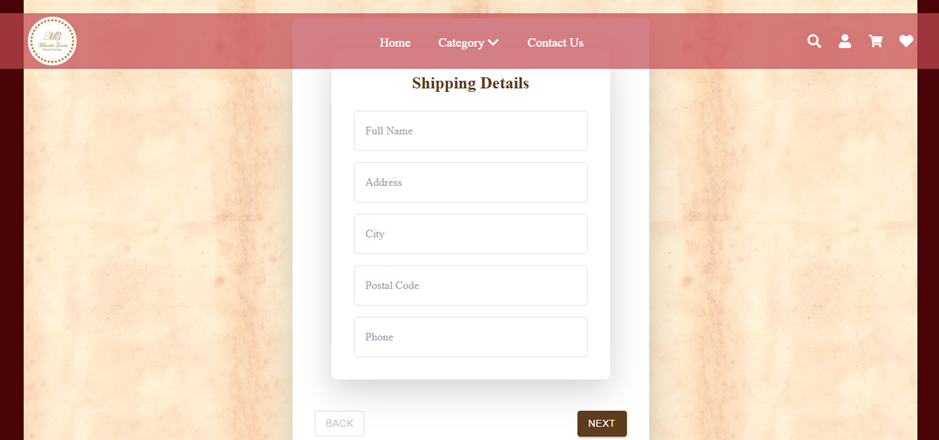
\includegraphics{images/Shipping details page.png}
\end{center}
\caption{Shipping details page}
\end{figure}

\newpage
\textbf{Order Summary:}\\

The Order Summary section provides a clear overview of the customer's selected items before finalizing the order. It displays each pastry added to the cart along with its name, quantity, individual price, and subtotal. Below the itemized list, the section also shows the total cost. This transparent breakdown allows users to review their order carefully and make any necessary adjustments before proceeding to payment, ensuring accuracy and confidence in the checkout process.

\begin{figure}[!h]
\begin{center}
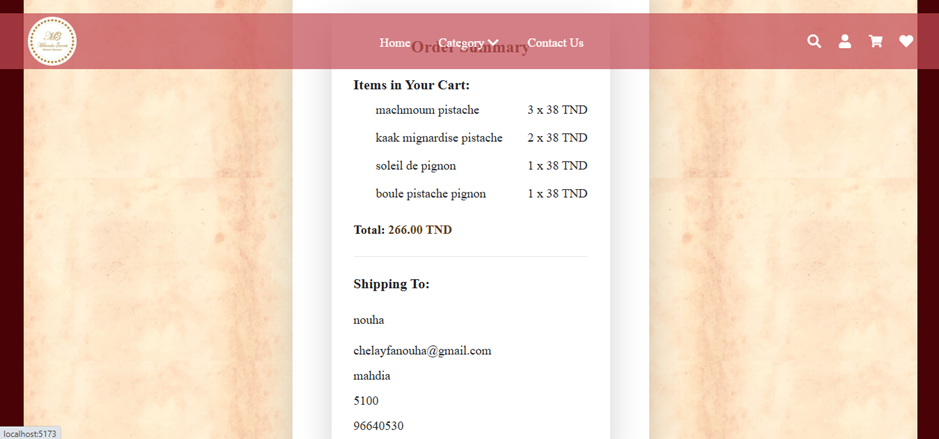
\includegraphics{images/Order Summary.png}
\end{center}
\caption{Order summary page}
\end{figure}

\textbf{Payment:}\\

The Payment section allows customers to pay using the local payment solution Monétique. Once a the pay now button is pressed, users are guided through a secure process to complete the transaction. This component ensures that payment details are handled safely and that the order is only confirmed once the payment is successfully processed, providing a reliable and trustworthy experience for every purchase.

\begin{figure}[!h]
\begin{center}
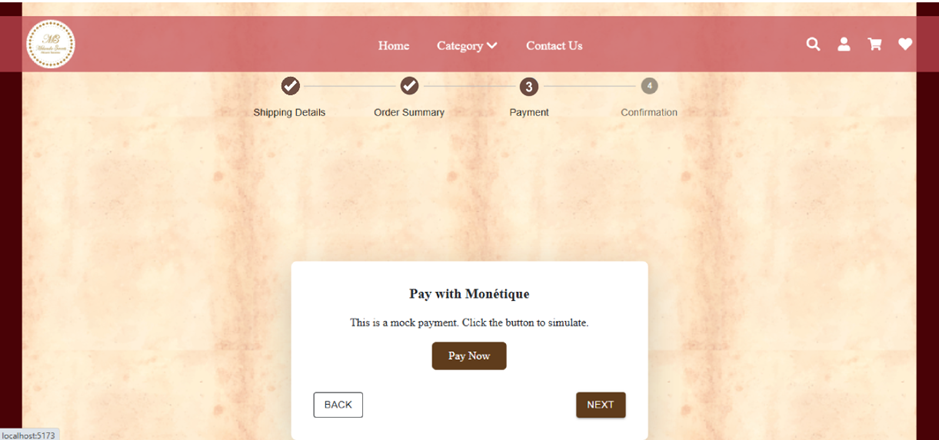
\includegraphics{images/Payment page.png}
\end{center}
\caption{Payment page}
\end{figure}

\newpage
\textbf{Confirmation:}\\

The Confirmation section finalizes the checkout process by reassuring the customer that their order has been successfully placed. It displays a warm thank-you message along with a unique order number, a summary of the items purchased, the total payment. This step confirms that the order is being processed and provides all essential details for reference.

\begin{figure}[!h]
\begin{center}
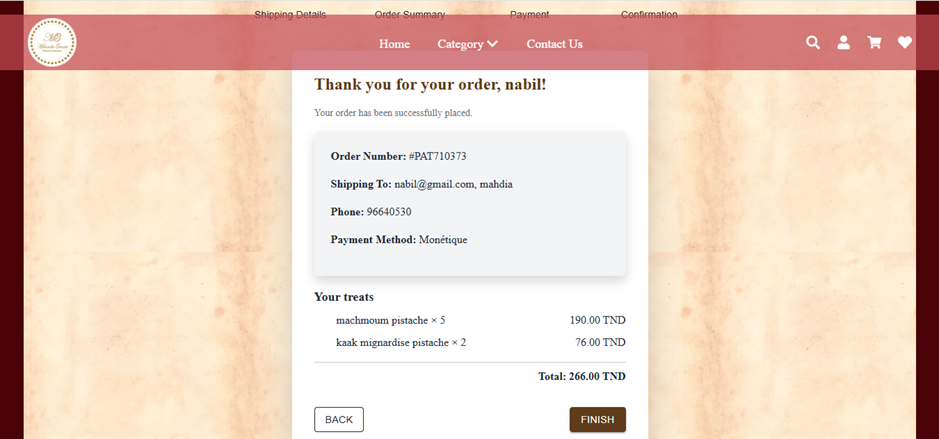
\includegraphics{images/Confirmation page.png}
\end{center}
\caption{Confirmation page}
\end{figure}

Once the user presses the ‘Finish’ button , a thank you for your order will be displayed and the user will get redirected to the homepage.

\begin{figure}[!h]
\begin{center}

\includegraphics{images/Homepage redirection.png}
\end{center}
\caption{Homepage redirection}
\end{figure}

\newpage
\section{Dashboard Interfaces:}

\subsection{Admin dashboard:}

The Admin Dashboard provides a centralized interface for managing the pastry shop’s online operations. Designed exclusively for authorized personnel, it offers a comprehensive overview of key business data and access to essential management tools. From here, admins can monitor orders, manage products, view customer activity, and track performance metrics. The dashboard is structured into modular sections, each dedicated to a specific task, enabling efficient day-to-day management and data-driven decision-making.

\begin{figure}[!h]
\begin{center}
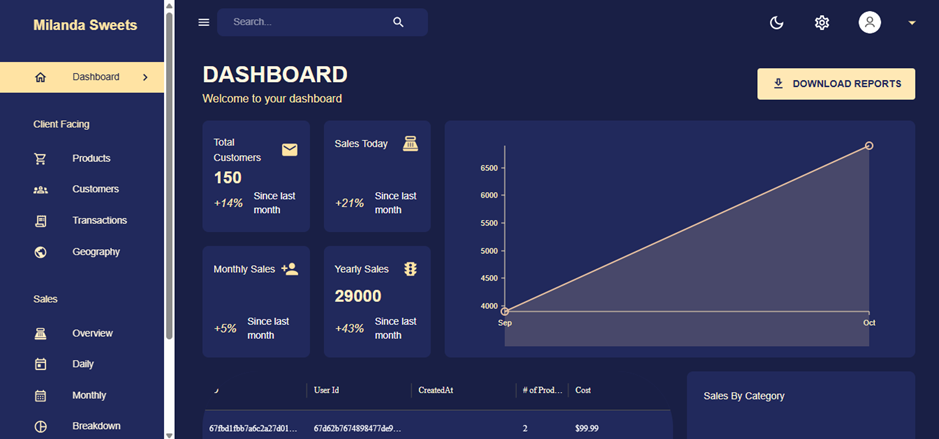
\includegraphics{images/Admin dashboard dark mode.png}
\end{center}
\caption{Admin dashboard dark mode}
\end{figure}

\begin{figure}[!h]
\begin{center}
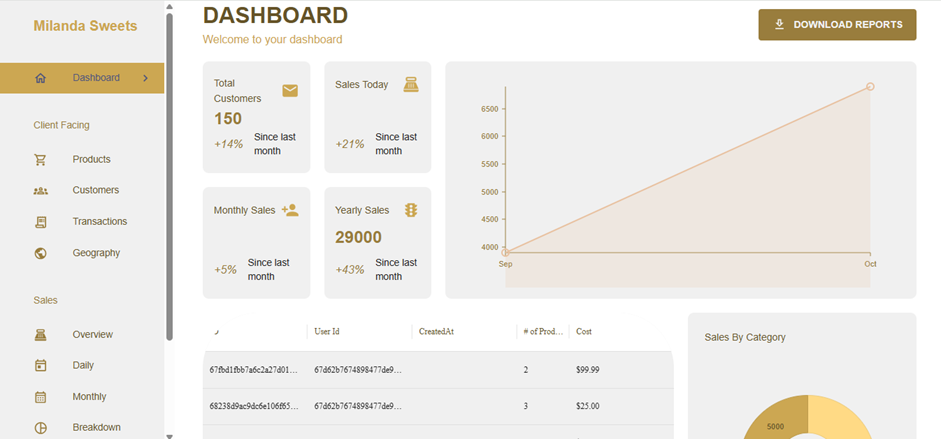
\includegraphics{images/Admin dashboard light mode.png}
\end{center}
\caption{Admin dashboard light mode}
\end{figure}

\newpage
\subsection{Products management page:}

The Product Management section allows admins to efficiently manage the pastry shop’s inventory and product offerings. This area provides an intuitive interface for adding new products, updating existing ones, and categorizing items by type .Admins can edit product details such as name, description, pricing, ingredients, stock levels, and images. Additionally, this section provides the ability to activate or deactivate products based on availability, ensuring the product catalog is always up-to-date and accurate for customers.

\begin{figure}[!h]
\begin{center}
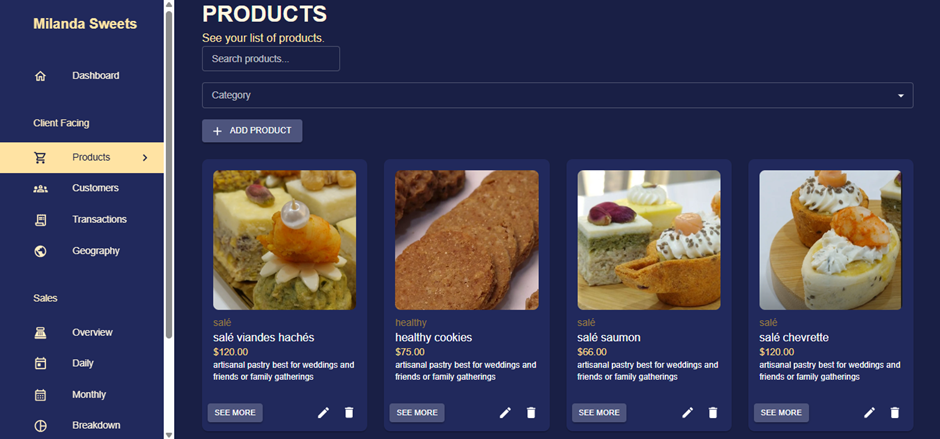
\includegraphics{images/Products management page.png}
\end{center}
\caption{Products management page}
\end{figure}

\subsection{Customers management page:}

The Customer Management section provides admins with tools to oversee and manage the shop’s customer base. This area allows admins to view a list of all registered customers, with details .Admins can search, filter, and sort through customer data to address specific needs or concerns.

\begin{figure}[!h]
\begin{center}
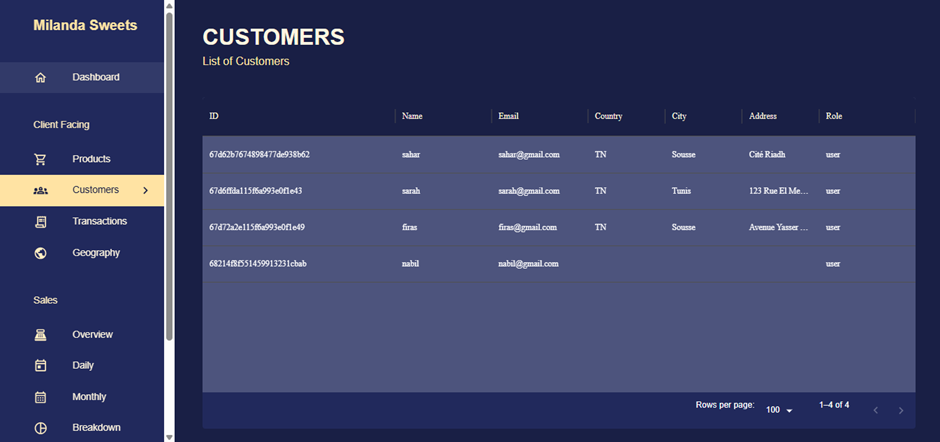
\includegraphics{images/Customers management page.png}
\end{center}
\caption{Customers management page}
\end{figure}

\newpage
\subsection{Transaction management page:}

The Transactions page offers a detailed overview of all financial transactions within the pastry shop’s online store. Admins can view each transaction's details, including order ID, customer information, product details, cost, and transaction dates.

\begin{figure}[!h]
\begin{center}
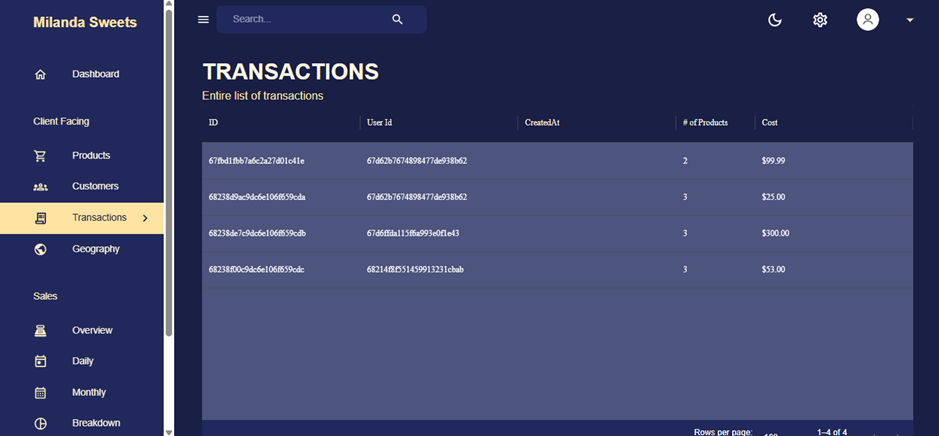
\includegraphics{images/Transaction management page.png}
\end{center}
\caption{Transaction management page}
\end{figure}

\subsection{Overview page:}

The Overview page provides admins with a high-level summary of key performance metrics. This page aggregates essential data in a form of a chart that showcases the total units per year as well as total sales per year . It serves as the central hub for understanding the overall health of the business and prioritizing actions accordingly.

\begin{figure}[!h]
\begin{center}
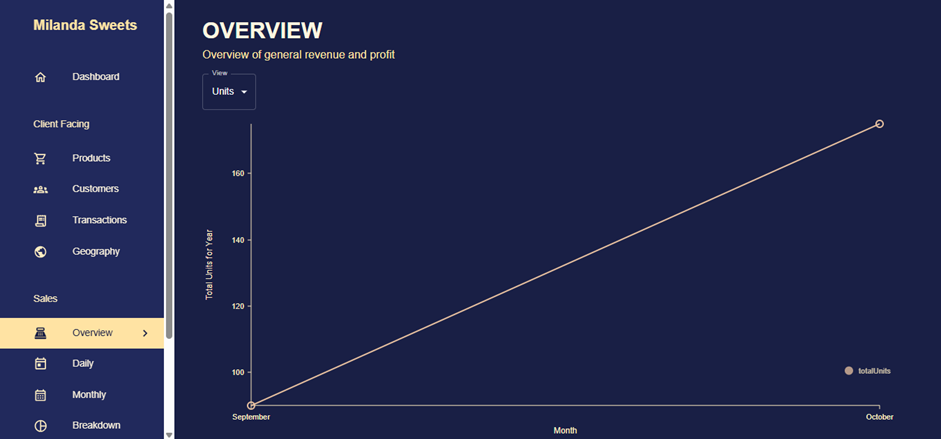
\includegraphics{images/Overview page.png}
\end{center}
\caption{Overview page}
\end{figure}

\newpage
\subsection{Daily sales page:}

The Daily Sales section provides a detailed breakdown of the pastry shop’s sales performance on a daily basis. Admins can view total sales on the daily in a form of a chart helping him track trends and spot any anomalies or significant changes in sales and easily monitor sales performance, assess the impact of promotions or special events, and make timely adjustments to business strategies.

\begin{figure}[!h]
\begin{center}
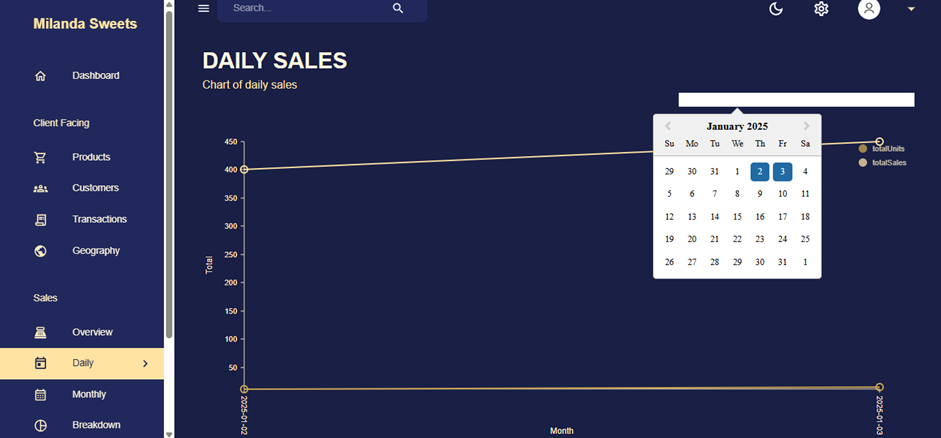
\includegraphics{images/Daily sales page.png}
\end{center}
\caption{Daily sales page}
\end{figure}

\subsection{Monthly sales page:}

The Monthly Sales section provides a comprehensive overview of the pastry shop's performance over the course of a month. Admins can view total sales, revenue, and order volume for each month, along with insights into trends and patterns through a chart. This section allows for easy comparison of current month’s data to previous months, highlighting growth, seasonal fluctuations, or the effectiveness of promotions. This approach helps admins track monthly progress, forecast future trends, and make informed decisions for upcoming sales strategies.

\begin{figure}[!h]
\begin{center}
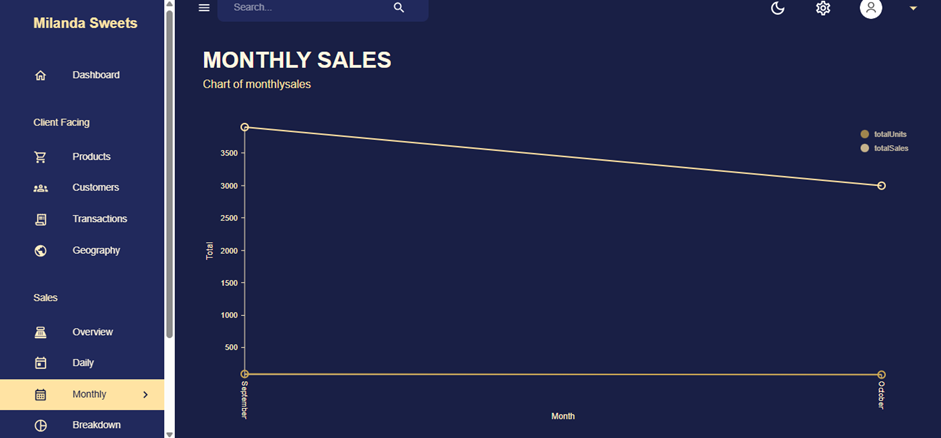
\includegraphics{images/Monthly sales page.png}
\end{center}
\caption{Monthly sales page}
\end{figure}

\subsection{Breakdown of sales page:}

The Breakdown section offers an in-depth analysis of sales and performance data, segmented product category. This section provides granular insights into what drives the business, helping admins identify popular products, assess payment trends, and better understand customer behavior which makes evaluating specific segments of the business and optimize strategies accordingly easier.

\begin{figure}[!h]
\begin{center}
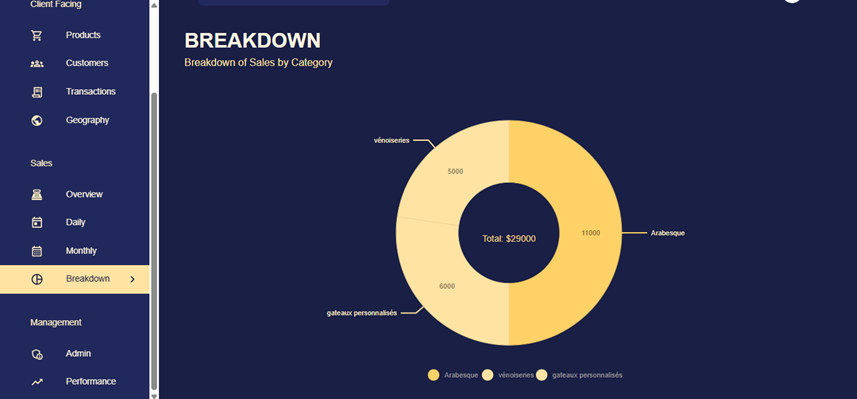
\includegraphics{images/Breakdown of sales page.png}
\end{center}
\caption{Breakdown of sales page}
\end{figure}

\subsection{Admin management page:}

The Admin Management section allows the primary administrator to oversee and manage other users with administrative access. This section enables the creation, modification, and deletion of admin accounts, assigning specific roles and permissions based on the responsibilities of each admin. Admins can set access levels, ensuring that different team members have appropriate control over various aspects of the platform, such as product management, order processing, or analytics. This helps maintain security, accountability, and streamlined operations within the team, providing flexibility while controlling who can access sensitive areas of the system.

\begin{figure}[!h]
\begin{center}
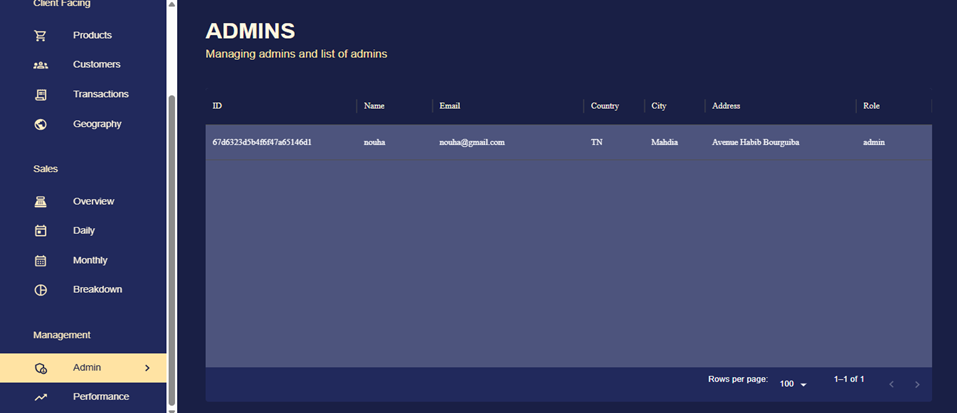
\includegraphics{images/Admin management page.png}
\end{center}
\caption{Admin management page}
\end{figure}

\newpage
\addcontentsline{toc}{section}{Conclusion}
{\Large \textbf{Conclusion:}}\\

In this final chapter, we completed the implementation phase by detailing the work environments, tools, and technologies used. To summarize this end-of-studies project, we conclude this report with a general overview and outline the potential future developments and perspectives.\\

\newpage
\addcontentsline{toc}{section}{Conclusion and Perspectives}
\begin{center}
    {\huge \textbf{Conclusion and Perspectives}}\\
\end{center}

\vspace{1cm} 

During this end-of-year project, we developed a complete eCommerce solution for the Patisserie Artisanal Tunisienne, aiming to provide a seamless online shopping experience for customers and a powerful management tool for the business.\\

The platform allows users to browse and order a variety of artisanal pastries, manage their carts, track orders, and securely complete their purchases. On the administrative side, it offers robust tools for managing products, orders, users, categories, and sales analytics, all from a centralized dashboard.\\

This report is structured in three chapters, each presenting a key phase of the project, The first chapter focused on the preliminary research and analysis, where we examined existing solutions, identified gaps, and defined the functional and non-functional requirements of our system. The second chapter covered the design and conception of the application, including its architecture, data modeling, user flows, and component interactions. The third chapter detailed the implementation phase, outlining the chosen technologies, development tools, and frameworks used to bring the solution to life. This section also included screenshots illustrating the main features and interfaces of the application.\\

Throughout the development process, we acquired valuable technical skills, deepened our understanding of full-stack web development, and gained hands-on experience in solving real-world business problems.
While this project successfully met its initial objectives, there are still opportunities for improvement and future development. Some key features that could enhance the solution include:

\begin{itemize}[label=\textbullet]
    \item \textbf{Mobile Application:} Extending the platform to mobile devices for better customer accessibility.
    \item \textbf{Live Order Tracking:}Providing customers with real-time updates on their order status and delivery progress.
    \item \textbf{Advanced Marketing Tools:} Integrating promotions, email marketing, and personalized product suggestions.
    \item \textbf{Multi-language Support:} Expanding accessibility to a wider audience by supporting additional languages.
    \item \textbf{Customer Reviews and Ratings:} Allowing users to share feedback on products and overall experience.
\end{itemize}

In conclusion, this project marked a significant step toward digital transformation for the pastry shop, laying a solid foundation for future growth and innovation.

\newpage
\addcontentsline{toc}{section}{Webography}
\begin{center}
    {\huge \textbf{Webography}}\\
\end{center}

\vspace{1cm}


\begin{itemize}
  \item [\textbf{[1]}] \href{https://masmoudi.tn}{https://masmoudi.tn}
  \item [\textbf{[2]}] \href{https://www.gourmandise.com.tn}{https://www.gourmandise.com.tn}
  \item [\textbf{[3]}] \href{https://patisserie-rekik.com}{https://patisserie-rekik.com}
  \item [\textbf{[4]}] \href{https://react.dev}{https://react.dev}
  \item [\textbf{[5]}] \href{https://expressjs.com}{https://expressjs.com}
  \item [\textbf{[6]}] \href{https://Tailwind.com}{https://Tailwind.com}
  \item [\textbf{[7]}] \href{https://Mongoose.com}{https://Mongoose.com}
  \item [\textbf{[8]}] \href{https://nodejs.org}{https://nodejs.org}
  \item [\textbf{[9]}] \href{https://GitHub.com}{https://GitHub.com}
  \item [\textbf{[10]}] \href{https://www.postman.com}{https://www.postman.com}
  \item [\textbf{[11]}] \href{https://Lucidchart.com}{https://Lucidchart.com}
  \item [\textbf{[12]}] \href{https://Visual.Studio.Code}{https://Visual.Studio.Code}
  \item [\textbf{[13]}] \href{https://www.mongodb.com}{https://www.mongodb.com}
\end{itemize}


\end{document}